\documentclass[12pt]{article}
%\usepackage{tocloft}% to configure the ToC <<<<<
%\setlength{\cftsecnumwidth}{4.5ex}% set the width to the section number in the ToC <<<<<
%\renewcommand{\thesection}{\Roman{section}.} 
%\renewcommand{\thesubsection}{\quad \Alph{subsection}.}
%\renewcommand{\thesubsubsection}{\qquad \roman{subsubsection}.}

%\usepackage[style=authoryear,bibencoding=auto,strict,backend=biber,natbib,maxcitenames=2]{biblatex}

\usepackage{amssymb,amsmath,amsfonts,bbm,bm,dcolumn,booktabs,eurosym,geometry,ulem,graphicx,color,xcolor,setspace,sectsty,comment,float,caption,pdflscape,subfigure,array,hyperref}
\usepackage{xurl}
\usepackage[font=bf]{caption}
\usepackage[bottom]{footmisc}

\hypersetup{
    colorlinks,
    linkcolor={black},
    citecolor={blue!35!black},
    urlcolor={blue!35!black}
}
\normalem
\interfootnotelinepenalty=10000

\geometry{left=1.0in,right=1.0in,top=1.0in,bottom=1.0in}

\usepackage[backend=bibtex]{biblatex}
\addbibresource{biblio.bib}

\begin{document}
\title{Assessing the Usefulness of News Sentiment for Real-Time Airline Stock Prediction}
\author{Steven VanOmmeren\thanks{A complete replication package of this project is available at \url{https://github.com/svanomm/svo-directed-practicum}.}}
\date{\today}
\maketitle
\begin{abstract}
\noindent
    The commercial airline industry is somewhat unique in that information about adverse events streams nearly 24/7/365, is highly publicized, and has potential to dramatically affect public trust in the company. In today's digital world, news of a fatal plane crash typically appears online within an hour. Knowledge of a plane crash or other adverse event could significantly impact the airline's stock price, either because the event reveals additional information to the public or because traders think that the event will matter. In addition, the general lack of after-hours trading for U.S. commercial airline stock allows real-time news sentiment to anticipate stock market movements.
    
    I examine the impact of such events on airline stock prices at the near-real-time level. Specifically, I leverage data from the Global Database of Events, Language, and Tone (GDELT) to scrape a rich set of sentiment measures from 1.3 million news articles mentioning the major U.S. commercial airlines. I use these (and other) data to predict changes in stock prices and volumes for 7 major U.S. airlines in 15-minute increments during the trading days from January 2018 to May 2025.

    I use GDELT data to identify adverse news events in real-time, reporting several event studies of news sentiment measures on stock prices/volumes for the respective airline. More generally, I explain and discuss the economic value of GDELT for business monitoring, which has applications outside the airline industry. 

    Combining my data with advanced machine learning techniques like Recurrent Neural Networks (RNN), Long Short-Term Memory (LSTM), Convolutional Neural Networks (CNN), LightGBM, and [[TBD...]], I am able to predict real-time stock volumes more accurately than state-of-the-art (SOTA) models in the literature. 

    This paper appears to be the first to publicly examine such a large volume of real-time GDELT data, the first to examine the effects of news sentiment on stock prices at a sub-daily level in the airline industry, and the first to consider the large set of supplemental sentiment indicators offered by GDELT for stock prediction. My analysis uses data that is at least an order of magnitude larger than most others, which provides additional assurances in the machine learning results (which require large-scale data for asymptotic guarantees). Finally, all of my code used to scrape and examine GDELT is available free and open-source, and can be used for business monitoring going forward.
\end{abstract}
\doublespacing
\section{Introduction}

GDELT.\footnote{\cite{leetaru2013gdelt}.}
\section{Literature Review}
\subsection{GDELT}
Previous studies have assessed the usefulness of GDELT for predicting stock prices. However, apparently all of them have aggregated GDELT to a daily level, rather than using it at its original real-time 15-minute increments. To my knowledge, only one study has taken advantage of the GDELT sentiment measures outside of the basic metrics of Tone, count of articles, and number of positive/negative sentiment words for predict financial markets.

\cite{nashir2023indonesian} incorporate GDELT data into a machine learning model to predict stock prices. The authors source a long span of daily stock data from Jan. 2008 to Dec. 2022 (5479 observations), specifically for the Jakarta Stock Exchange (JKSE) index of Indonesian stocks. The authors study 4 sentiment measures using GDELT data: tone, optimism, attention, and tone dispersion. These metrics are calculated at the daily level. The authors then train a modified version of an LSTM model using time series cross-validation. The authors document an extensive hyperparameter optimization, which yielded an improved model with a mean absolute percentage error (MAPE) of 0.8\%. They additionally find that a model trained with only the ``optimism" feature slightly outperforms the model with all four sentiment measures.\footnote{The combined model outperforms the other models that include only a single sentiment metric (tone, attention, or tone dispersion).} The authors do not compare their results to a Naive forecast.

\cite{wang2024ensemble} use GDELT data to inform the prediction of a variety of individual stocks and indices. They do not identify articles specific to each stock, instead summing the number of article mentions and the sum of Tone for each CAMEO code. CAMEO codes provide high-level descriptions of conflict identified in an article, e.g. ``Threaten" or ``Engage in political dissent." The authors then evaluate causal relationships between the CAMEO-specific metrics with each stock price at the daily level from Jan. 2018 to Feb. 2022. These causal relationships are incorporated into an LSTM model to predict stock prices. The authors report that this model performs best out of a variety of other models (including ARIMA, VAR, etc.). Unfortunately, the authors do not compare the performance of their model to a Naive prediction, and a close look at their Figures 9 and 10 shows that their best model essentially predicts the previous stock price. In other words, they likely do not beat a Naive forecast.

\cite{consoli2021information} assess the use of GDELT for modeling sovereign spreads in the European bond market. The time series of interest is the sovereign spread of Italy vs Germany with respect to 10-year bond yields, with 468 data points covering a time period of Mar. 2015 to Aug. 2019. The authors filtered GDELT to identify articles specific to macroeconomic discussions in the locations of interest. They identify a subset of 45 GDELT variables that are both quantitatively and qualitatively relevant to bond markets. The authors then include these variables along with bond market data in a probabilistic LSTM model, yielding an out-of-sample R-squared of 0.23 for predicting changes in the dependent variable. While the study suffers from a small sample size and does not compare its accuracy to a Naive forecast, it provides robust evidence that GDELT could be useful for predicting bond markets.

\cite{jakel2019using} investigates correlations between GDELT sentiment and the stock prices of U.S. technology companies. The author sourced approximately 60,000 articles over a 29-day period in 2019. He then averaged the sentiment Tone by company and day to join to 29 days of stock price data for Facebook, Apple, Amazon, Alphabet and Tesla. Analyzing the correlation between sentiment and stock price, the author found a generally contrarian relationship. However, the results are inconclusive due to a small sample size.

\cite{alamro2019predicting} use GDELT's Tone and count of articles per day to predict TASI, a Saudi stock market index. The authors filtered GDELT data to any articles that mention Saudi Arabia, then aggregate the data to the daily level, averaging the Tone metric and counting the number of articles per day. The authors then test a variety of models to predict the index price, finding that an LSTM model performs dramatically better than more traditional forecasting models. Unfortunately, the authors do not report the specification of the LSTM model, any scale-independent measures of model fit, any comparisons to a Naive forecast, any tests of whether the sentiment measures add predictive value, nor any graphs of predicted vs actual stock prices. It is therefore unclear whether the authors' LSTM model provides better-than-Naive performance or if the sentiment measures actually improved the fit of the model.

\subsection{Airline Stock Prediction}
\cite{kaplanski2010sentiment} study the short-run effects of major airline disasters on the stock market at large. They identify 288 aviation disasters over a 58-year period and analyze the average change in NYSE Composite Index returns in the days that follow each disaster. The authors find that, on average, there is a noticeable decrease in market returns the day after an airline disaster. Following a sharp decrease in the first two days, the market returns to normal after approximately 2 weeks. They show that the lost value in the stock market is over 60 times larger than the economic loss incurred by the disaster. These results support the idea that anxiety-inducing events can have an outsized effect on the market.

\subsection{Stock Volume Prediction}
The fact that most traders are concerned with predicting stock prices makes stock prices nearly impossible to predict. An average day trader with access to the same (or worse) stock data as everyone else in the market is almost certainly unable to predict prices better than a firm employing hundreds or thousands of Ph.Ds to do predictions full-time. However, predicting trading volumes (which do not provide direct information of prices) is a more attainable problem.

\cite{goyenko2024trading} model the potential benefits associated with accurate predictions of trading volume. The authors explain that while trading volume is not particularly useful to a day trader, inaccurate forecasts of volume could lead a large trading firm to miscalculate the price impact of a trade. In the authors' theoretical model, overestimating the amount of trading volume when making a large trade would increase the net trading cost to the firm. The authors create a predictive model of changes in the log of dollar trading volume using technical indicators for 4700 stocks over a period of 1258 days. Relative to the prediction accuracy of a moving average model, their best model (an LSTM with 175 features) obtains a relative $R^2$ of around 20\%. This demonstrates that, unlike stock price prediction, models can consistently predict daily trading volumes over a wide range of stocks.

\cite{cucuringu2025forecasting} investigate the ability of machine learning models to predict intraday trading volumes. The authors analyze 15-minute data over a period of 6 months for each constituent stock in the S\&P 500 index. A baseline model is able to predict out-of-sample volumes with an $R^2$ of 0.265, while their best model attains an $R^2$ of 0.624. The authors then demonstrate the usefulness of their model for large traders seeking to minimize the price impact of a trade. Their model improves the volume-weighted average price (VWAP) order execution risk for a sample of 5 stocks by an average of around 29\%, compared to a baseline model.

\cite{satish2014predicting} make the case for using a statistical model to predict trading volumes. The authors explain that at the time,  the typical approach taken by firms was to just use moving averages of trading volumes as a predictor. The authors combine two ARMA models with varying levels of historical data (intraday and daily) to predict trading volume. After calibrating their model, the authors were able to increase VWAP error performance by 9\% compared to the typical moving average approach. Notably, the authors explain that news events can affect VWAP tracking error, though they do not include news sentiment in their model.

\section{Methods}
Below, I explain the data preparation and modelling techniques used to evaluate the usefulness of GDELT for predicting airline stocks.\footnote{All processing and modelling was performed on a Windows 10 desktop with the following specifications: 128GB of DDR4 RAM, an Nvidia RTX 2070 Super (8GB VRAM), and an AMD Ryzen 5 3600 processor. Some of the computations described below likely would not run on anything less than 128GB of RAM without modification.}
\subsection{Data Preparation}
\subsubsection{GDELT}
GDELT offers a variety of databases to the public. For this analysis, I used the Global Knowledge Graph version 2 (GKG). For each article identified by GDELT, the GKG reports:
\begin{itemize}
\singlespacing
    \item the date scraped by GDELT (at the 15-minute level)
    \item the article URL (or other unique identifier)
    \item every location, business, and important person named in the article text
    \item Conflict and Mediation Event Observations (CAMEO) codes identified in the article
    \item 7 sentiment measures based on the article text (Tone, Positive Score, Negative Score, Polarity, Activity Reference Density, Self/Group Reference Density, Word Count). These are called the GKG1 sentiment measures
    \item 111 additional sentiment measures that use a scored value (called the GKG2 scored measures)
    \item 2878 additional sentiment measures that use word count (called the GKG2 word count measures)
    \item the article headline text (if available)\footnote{GDELT only started scraping the article headline in Sep. 2019. Prior to this time, I was able to scrape part of the article headline using the URL, which often contains a relevant description of the story.}
\end{itemize}
Importantly, GDELT does \textit{not} store the article text itself. GDELT uploads the raw GKG data in separate files every 15 minutes. These files are available to download for free, but the full combined data is available to query in Google BigQuery for a fee. The files are saved at the article level, i.e. the articles that GDELT scraped in a given 15-minute period.

Because the combined data is several (if not more) terabytes (TBs), I did not have the storage capacity to save all the raw data. Instead, I filtered the raw files to articles matching the airline industry before saving the data. The general outline of my data processing is:
\begin{itemize}
\singlespacing
    \item access and unzip the raw file for a given 15-minute period
    \item keep a limited subset of columns from the raw file to save space
    \item limit to articles mentioning a location of ``United States"
    \item limit to articles that mention at least one of the following organizations: Alaska Airlines, American Airlines, Delta Air Lines, Frontier Airlines, Hawaiian Airlines, JetBlue, Southwest Airlines, Spirit Airlines, Sun Country Airlines, United Airlines, Allegiant Air
    \item drop articles that are missing any key fields
\end{itemize}
I repeated this process for the approximately 260,000 15-minute periods covering the timeline of 1/1/2018 00:00:00 to 5/30/2025 23:45:00. Data downloading was performed over multiple several-hour periods, and was parallelized to increase download speeds. After filtering, 218,574 raw GDELT files were combined for a total of 1,261,785 articles identified.\footnote{The total raw GDELT files kept is less than the theoretical 260,000 files for multiple reasons, including: no airlines mentioned in the past 15 minutes, and sporadic GDELT outages.}

Next, I performed extensive data cleaning to filter out irrelevant articles from the data:
\begin{itemize}
\singlespacing
    \item removing frequent article titles that relate to the front page of a news site (rather than a specific article) or an unrelated article
    \item removing certain websites that are unlikely to contain relevant articles (for example websites that discuss airline points programs)
    \item removing discussions of historical airline events (such as the September 11 attacks)
    \item removing articles that did not have a valid article title after data processing
    \item removing a small set of duplicate articles\footnote{Duplicate articles are likely due to my data downloading process, which was stopped and restarted multiple times.}
\end{itemize}
After cleaning, we have 1,121,056 relevant articles.

The processed GDELT data has 2,996 sentiment measures in total. However, some of the measures contained no information for the subset of data and were dropped.\footnote{Example column: ``c31.5; WORDCOUNT; EMOTION/GLORY." ``No information" means that the column's minimum and maximum values are the same.} After dropping there are 7 GKG1 measures, 40 GKG2 scored measures, and 2,410 GKG2 word count
measures. To reduce the variable count, we use \textbf{Principal Components Analysis} (PCA).

PCA is a dimensionality reduction technique that identifies orthogonal linear combinations of variables that maximize the explained variance in a dataset. Limiting to a subset of these principal components is akin to compressing the size of the data in the ``best'' linear way possible. In this case, I used PCA separately on the three subsets of variables.\footnote{For the GKG2 word count measures, I used incremental PCA with a batch size of 200,000 observations due to RAM limitations on my computer.} Before running PCA, each column was rescaled to have mean zero and unit variance. The scree plots below report the cumulative variance explained by the first $n$ principal components.

Of the 40 GKG2 scored measures, the first 5 principal components explain $\approx 70\%$ of the variance. Of the 2,410 GKG2 word count measures, the first 5 principal components explain $\approx 64\%$ of the variance.

After calculating the principal component vectors, I then evaluated the first [[5]] components from each subset on the full dataset, for a total of 15 sentiment measures.\footnote{This is a computationally intensive operation for the GKG2 word count measures. Evaluating a single principal component on the data requires multiplying floating-point matrices of size $(1121056,2410)$ and $(2410,1)$.}

As a supplemental sentiment measure, I evaluated a \textbf{Large Language Model} (LLM) on the article titles. For each article title, I apply a 67-million parameter embedding model.\footnote{\url{https://huggingface.co/tabularisai/robust-sentiment-analysis}.} This model outputs a vector of 5 numbers which represent the probability of the text belonging to a sentiment category: Very Negative, Negative, Neutral, Positive, Very Positive. I convert these probabilities into a single score by taking the dot product of the probability vector with the vector $(-2,-1,0,1,2)$, which yields a metric from $-2$ (Very Negative) to 2 (Very Positive).

After evaluating PCA at the article level, we need to aggregate the data to align with stock market data and to identify sentiment scores separately by airline. Each PCA metric, GKG1 measure, the LLM measure, and an Article Count metric are interacted with airline dummies. We then sum the metrics by  15-minute interval and fill in missing time periods with zeroes.\footnote{GDELT data is recorded in the UTC timezone, while my stock data is in EST. I converted the timezone before merging these datasets.}

At this point, the GDELT data is in 15-minute intervals, but it includes times outside of market open. We further aggregate the data to align with market open (9:30 to 15:45 in my data). The choice of aggregation strategy is not obvious here. The number of observations to aggregate influences the scale of the resulting sentiment scores. Summing a particular window of observations (e.g. 2 hours) assumes that sufficient information is captured in that time period for predicting stock behavior. I address this issue by calculating rolling sums over varying time windows: 1 hour, 2 hours, 4 hours, 12 hours, and 24 hours. These sums influence the non-after-hours observations as well, making them essentially moving averages. After calculating the rolling sums for each airline, metric, and window, I calculate the first difference of the variable.

\subsubsection{Stocks}
Stock data were downloaded in 15-minute increments during market open from Barchart, for the period Jan. 2018 to May 2025. The following tickers were downloaded:
\begin{itemize}
\singlespacing
    \item AAL: American Airlines Group Inc.
    \item ALGT: Allegiant Travel Company
    \item ALK: Alaska Air Group Inc.
    \item BNO: United States Brent Oil Fund LP
    \item DAL: Delta Air Lines Inc.
    \item ITA: iShares US Aerospace \& Defense ETF
    \item IYT: iShares US Transportation ETF
    \item JBLU: JetBlue Airways Corp.
    \item JETS: US Global Jets ETF
    \item LUV: Southwest Airlines Co.
    \item UAL: United Airlines Holdings Inc.
\end{itemize}
As seen from the list, I include some stocks as control variables that are likely correlated with airline stocks: 3 airplane-related ETFs, and an oil fund. The raw data include the stock's open, high, low, and last price, and volume traded over each 15-minute period. I calculate additional features for each stock:
\begin{itemize}
\singlespacing
    \item High-Low spread (in levels and percentage)
    \item Last-Open spread (in levels and percentage)
    \item 1-period change in open, high, low, last price, and volume
    \item Change in trading volume compared to same time on previous trading day
    \item 10-period rolling standard deviation of last price
    \item 10-period rolling standard deviation of volume
    \item 10-period rolling standard deviation of the 10-period SD of price
    \item 10-period rolling standard deviation of the 10-period SD of volume
\end{itemize}
The last 4 measures are meant to capture changes in volatility for a given stock. The daily change in trading volume is a better metric to analyze market opens and closes, as many of the airline stocks are traded heavily at 9:30 and 15:45, but have little volume for the rest of the day. 

I then calculate a variety of moving averages for each metric, with the following windows: 8 periods (2 hours), 16 periods (4 hours), 26 periods (one trading day), 52 periods (two trading days).

\subsubsection{Airlines}

\subsection{LightGBM}

\subsection{RNN}

\subsection{LSTM}

\subsection{CNN}

\subsection{Hyperparameter Tuning}
Hyperparameter tuning is the process of changing some of the input settings in the model to optimize its performance. I use a randomized grid search, in which parameters are randomly chosen from within a specified range, to test many possible combinations of settings. I then evaluate each combination by its predictive power on the test sets, and choose the model with the best performance. I varied the following parameters:

\subsubsection{Shapley Values}
The final model is extremely large and complex. Machine learning models are often described as being ``black boxes,'' with no possible way of understanding how or why they work. However, Shapley values provide some insight into the model. Shapley values are calculated by randomly selecting an observation, perturbing some of its features, and seeing how much the predicted sales changes as a result. We then repeat this procedure many thousands of times to get an understanding of how much each variable contributes to the final predicted value. I implemented the Shapley value calculations with the \textsf{shap} package in Python.\footnote{\cite{shap}.}

\subsection{Ensemble Models}

\section{Results and Analysis}
\subsection{Summary Analysis}
\subsection{Correlation Analysis}
\subsubsection{Contemporaneous Correlation}
First, Figure \ref{fig:contemp_open} reports the contemporaneous correlation in first-differences of open price for the airline stocks of interest. Correlations are calculated using the 15-minute data.
\begin{figure}[H]
    \centering
    \caption{Contemporaneous Correlation, Change in Open Price}
%    \includegraphics[width=0.75\linewidth]{Figures/Contemporaneous_Open.png}
    \label{fig:contemp_open}
\end{figure}
Next, Figure \ref{fig:contemp_vol} reports the contemporaneous correlation in first-differences of trading volume for the airline stocks of interest.
\begin{figure}[H]
    \centering
    \caption{Contemporaneous Correlation, Change in Trading Volume}
 %   \includegraphics[width=0.75\linewidth]{Figures/Contemporaneous_Volume.png}
    \label{fig:contemp_vol}
\end{figure}
These figures show that the airline stocks exhibit a substantial and positive correlation. The airline-relevant indices (ITA, IYT, and JETS) have lower but still-relevant positive correlations. 

\subsubsection{Lagged Correlation}
Next, I report the correlations among the lag of these variables. Figure \ref{fig:lagged_open} reports correlations between a stock's change in price at time $t$ (the rows) with a stock's change in price at time $t-1$ (the columns). For example, the diagonal entries report the first-order autocorrelation of each stock.
\begin{figure}[H]
    \centering
    \caption{Lagged Correlation, Change in Open Price}
 %   \includegraphics[width=0.75\linewidth]{Figures/Lagged_Open.png}
    \label{fig:lagged_open}
\end{figure}
Similarly, Figure \ref{fig:lagged_volume} reports the correlations among changes in trading volumes.
\begin{figure}[H]
    \centering
    \caption{Lagged Correlation, Change in Trading Volume}
%    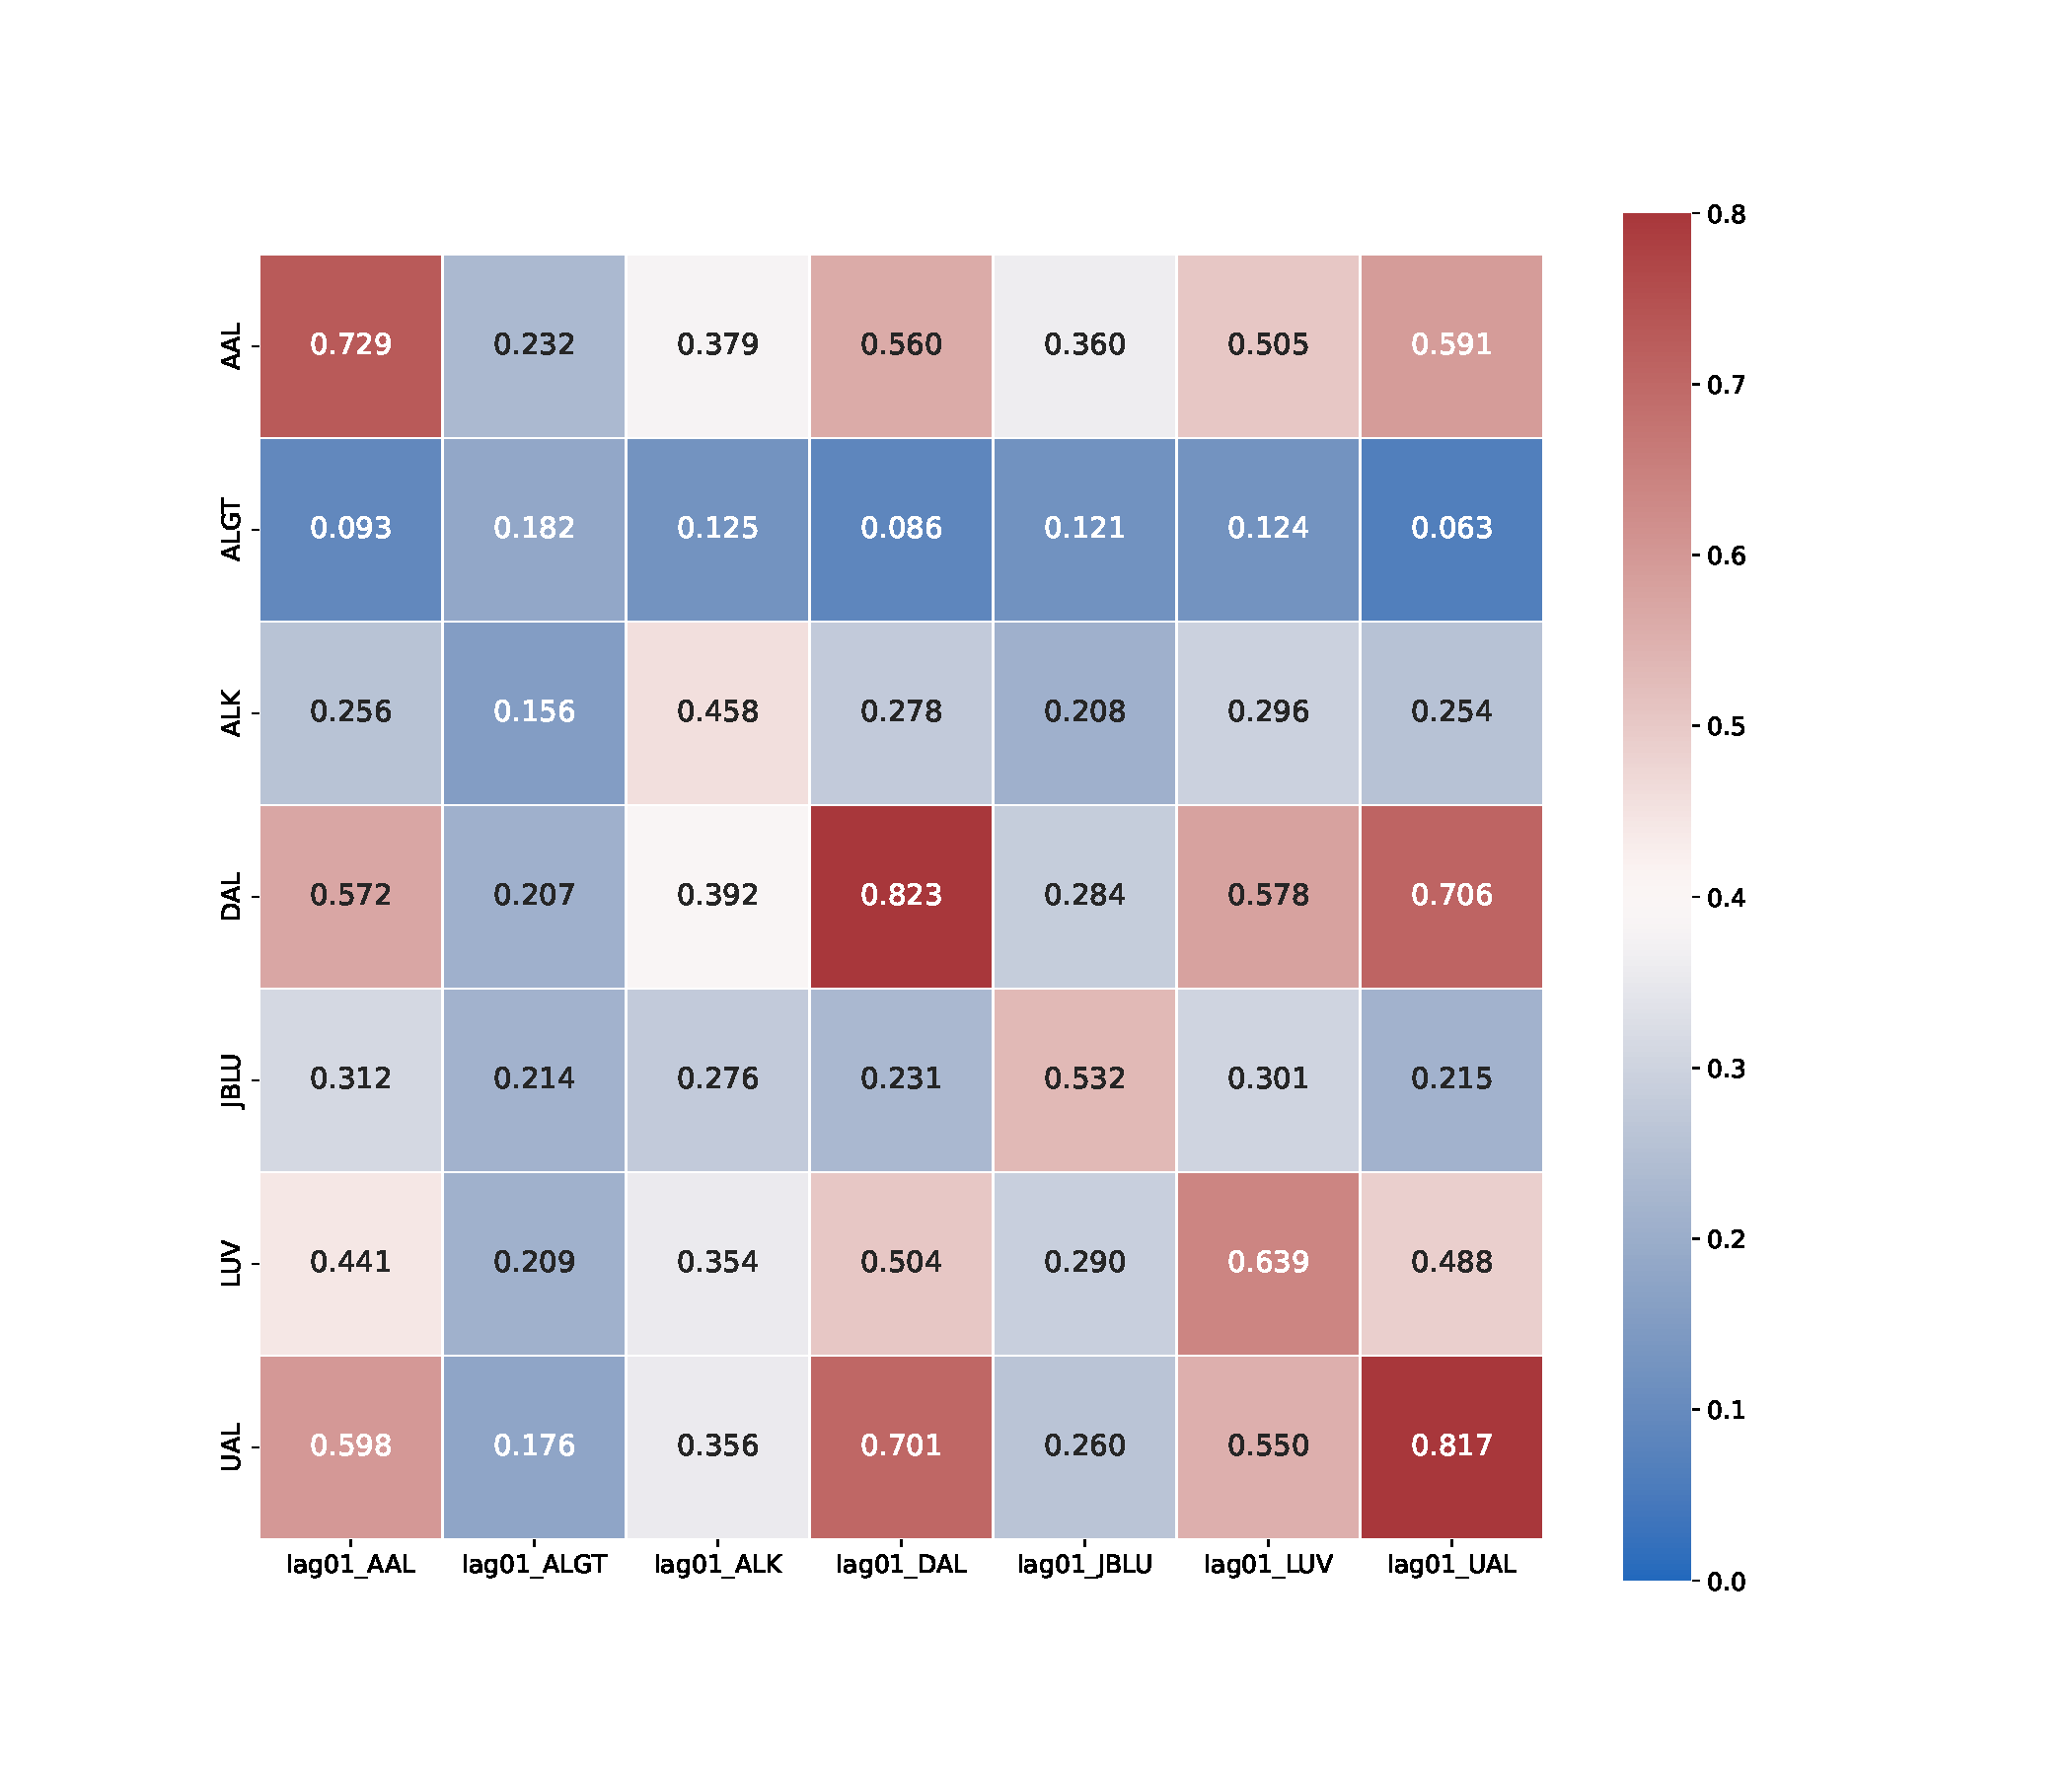
\includegraphics[width=0.75\linewidth]{Figures/Lagged_Volume.png}
    \label{fig:lagged_volume}
\end{figure}
Due to the highly unpredictable nature of the stock market, these correlations are much smaller. For example, United Airlines and Delta Airlines have a contemporaneous correlation of 0.83 with respect to price changes, but lagged price changes for Delta have only a 0.038 correlation with current price changes for United.

While the lagged correlations for prices are mostly positive, the lagged correlations in trading volume are almost all negative, a reversal compared to the contemporaneous chart.


\subsection{Models}

\newpage
\section{Discussion}

\section{Conclusion}

\newpage
\printbibliography
\end{document}